% Created 2021-12-24 Fri 23:08
\documentclass[9pt, b5paper]{article}
\usepackage[UTF8]{ctex}
\usepackage{xltxtra}
\usepackage{bera}
\usepackage[T1]{fontenc}
\usepackage[scaled]{beraserif}
\usepackage[scaled]{berasans}
\usepackage[scaled]{beramono}
\usepackage{graphicx}
\usepackage{xcolor}
\usepackage{multirow}
\usepackage{multicol}
\usepackage{float}
\usepackage{textcomp}
\usepackage{geometry}
\geometry{left=1.2cm,right=1.2cm,top=1.5cm,bottom=1.2cm}
\usepackage{algorithm}
\usepackage{algorithmic}
\usepackage{latexsym}
\usepackage{natbib}
\usepackage{minted}
\newminted{common-lisp}{fontsize=ootnotesize}
\usepackage[xetex,colorlinks=true,CJKbookmarks=true,linkcolor=blue,urlcolor=blue,menucolor=blue]{hyperref}
\author{deepwaterooo}
\date{\today}
\title{Kotlin Grammer}
\hypersetup{
  pdfkeywords={},
  pdfsubject={},
  pdfcreator={Emacs 27.1 (Org mode 8.2.7c)}}
\begin{document}

\maketitle
\tableofcontents


\section{空安全}
\label{sec-1}

\subsection{可空类型与非空类型}
\label{sec-1-1}
\begin{itemize}
\item Kotlin 的类型系统旨在消除来自代码空引用的危险,也称为《十亿美元的错误》。
\item 许多编程语言(包括 Java)中最常见的陷阱之一,就是访问空引用的成员会导致空引用异常。在 Java 中,这等同于 NullPointerException 或简称 NPE。
\item Kotlin 的类型系统旨在从我们的代码中消除 NullPointerException。NPE 的唯一可能的原因可能是:
\begin{itemize}
\item 显式调用 throw NullPointerException();
\item 使用了下文描述的 !! 操作符;
\item 有些数据在初始化时不一致,例如当:
\begin{itemize}
\item 传递一个在构造函数中出现的未初始化的 this 并用于其他地方(“泄漏 this”);
\item 超类的构造函数调用一个开放成员,该成员在派生中类的实现使用了未初始化的状态;
\end{itemize}
\item Java 互操作:
\begin{itemize}
\item 企图访问平台类型的 null 引用的成员;
\item 用于具有错误可空性的 Java 互操作的泛型类型,例如一段 Java 代码可能会向 Kotlin 的 MutableList<String> 中加入 null,这意味着应该使用 MutableList<String?> 来处理它;
\item 由外部 Java 代码引发的其他问题。
\end{itemize}
\end{itemize}
\item 在 Kotlin 中,类型系统区分一个引用可以容纳 null (可空引用)还是不能容纳(非空引用)。 例如,String 类型的常规变量不能容纳 null:
\end{itemize}
\begin{minted}[frame=lines,fontsize=\scriptsize,linenos=false]{kotlin}
var a: String = "ab"
var a: String = "abc" // 默认情况下,常规初始化意味着非空
a = null // 编译错误
\end{minted}
\begin{itemize}
\item 如果要允许为空,我们可以声明一个变量为可空字符串,写作 String?:
\end{itemize}
\begin{minted}[frame=lines,fontsize=\scriptsize,linenos=false]{kotlin}
var b: String? = "abc" // 可以设置为空
b = null // ok
print(b)
\end{minted}
\begin{itemize}
\item 现在,如果你调用 a 的方法或者访问它的属性,它保证不会导致 NPE,这样你就可以放心地使用:
\end{itemize}
\begin{minted}[frame=lines,fontsize=\scriptsize,linenos=false]{kotlin}
val l = a.length
\end{minted}
\begin{itemize}
\item 但是如果你想访问 b 的同一个属性,那么这是不安全的,并且编译器会报告一个错误:
\end{itemize}
\begin{minted}[frame=lines,fontsize=\scriptsize,linenos=false]{kotlin}
val l = b.length // 错误:变量“b”可能为空
\end{minted}
\begin{itemize}
\item 但是我们还是需要访问该属性,对吧?有几种方式可以做到。
\end{itemize}

\subsection{在条件中检测 null}
\label{sec-1-2}
\begin{itemize}
\item 首先,你可以显式检测 b 是否为 null,并分别处理两种可能:
\end{itemize}
\begin{minted}[frame=lines,fontsize=\scriptsize,linenos=false]{kotlin}
val l = if (b != null) b.length else -1
\end{minted}
\begin{itemize}
\item 编译器会跟踪所执行检测的信息,并允许你在 if 内部调用 length。 同时,也支持更复杂(更智能)的条件:
\end{itemize}
\begin{minted}[frame=lines,fontsize=\scriptsize,linenos=false]{kotlin}
val b: String? = "Kotlin"
if (b != null && b.length > 0) {
    print("String of length ${b.length}")
} else {
    print("Empty string")
}
// String of length 6
\end{minted}
\begin{itemize}
\item 请注意,这只适用于 b 是不可变的情况(即在检测和使用之间没有修改过的局部变量 ,或者不可覆盖并且有幕后字段的 val 成员),因为否则可能会发生在检测之后 b 又变为 null 的情。况
\end{itemize}

\subsection{安全的调用}
\label{sec-1-3}
\begin{itemize}
\item 你的第二个选择是安全调用操作符,写作 ?.:
\end{itemize}
\begin{minted}[frame=lines,fontsize=\scriptsize,linenos=false]{kotlin}
val a = "Kotlin"
val b: String? = null
println(b?.length)
println(a?.length) // 无需安全调用
\end{minted}
\begin{itemize}
\item 如果 b 非空,就返回 b.length,否则返回 null,这个表达式的类型是 Int?。
\item 安全调用在链式调用中很有用。例如,如果一个员工 Bob 可能会(或者不会)分配给一个部门, 并且可能有另外一个员工是该部门的负责人,那么获取 Bob 所在部门负责人(如果有的话)的名字,我们写作:
\end{itemize}
\begin{minted}[frame=lines,fontsize=\scriptsize,linenos=false]{kotlin}
bob?.department?.head?.name
\end{minted}
\begin{itemize}
\item 如果任意一个属性(环节)为空,这个链式调用就会返回 null。
\item 如果要只对非空值执行某个操作,安全调用操作符可以与 let 一起使用:
\end{itemize}
\begin{minted}[frame=lines,fontsize=\scriptsize,linenos=false]{kotlin}
val listWithNulls: List<String?> = listOf("Kotlin", null)
for (item in listWithNulls) {
    item?.let { println(it) } // 输出 Kotlin 并忽略 null
}
\end{minted}
\begin{itemize}
\item 安全调用也可以出现在赋值的左侧。这样,如果调用链中的任何一个接收者为空都会跳过赋值,而右侧的表达式根本不会求值:
\end{itemize}
\begin{minted}[frame=lines,fontsize=\scriptsize,linenos=false]{kotlin}
// 如果 `person` 或者 `person.department` 其中之一为空,都不会调用该函数:
person?.department?.head = managersPool.getManager()
\end{minted}

\subsection{Elvis 操作符}
\label{sec-1-4}
\begin{itemize}
\item 当我们有一个可空的引用 b 时,我们可以说“如果 b 非空,我使用它;否则使用某个非空的值”:
\end{itemize}
\begin{minted}[frame=lines,fontsize=\scriptsize,linenos=false]{kotlin}
val l: Int = if (b != null) b.length else -1
val l: Int = if (b != null) b.length else -1
\end{minted}
\begin{itemize}
\item 除了完整的 if-表达式,这还可以通过 Elvis 操作符表达,写作 ?::
\end{itemize}
\begin{minted}[frame=lines,fontsize=\scriptsize,linenos=false]{kotlin}
val l = b?.length ?: -1
val l = b?.length ?: -1
\end{minted}
\begin{itemize}
\item 如果 ?: 左侧表达式非空,elvis 操作符就返回其左侧表达式,否则返回右侧表达式。 请注意, \uline{当且仅当左侧为空时,才会对右侧表达式求值。}
\item 请注意, \uline{因为 throw 和 return 在 Kotlin 中都是表达式,所以它们也可以用在 elvis 操作符右侧。这可能会非常方便,例如,检测函数参数:}
\end{itemize}
\begin{minted}[frame=lines,fontsize=\scriptsize,linenos=false]{kotlin}
fun foo(node: Node): String? { // <<<==== 返回值可为空
    val parent = node.getParent() ?: return null
    val name = node.getName() ?: throw IllegalArgumentException("name expected")
    // ……
}
\end{minted}

\subsection{!! 操作符: 非空断言运算符(!!)}
\label{sec-1-5}
\begin{itemize}
\item 第三种选择是为 NPE 爱好者准备的:非空断言运算符(!!)将任何值转换为非空类型,若该值为空则抛出异常。我们可以写 b!! ,这会返回一个非空的 b 值 (例如:在我们例子中的 String)或者如果 b 为空,就会抛出一个 NPE 异常:
\end{itemize}
\begin{minted}[frame=lines,fontsize=\scriptsize,linenos=false]{kotlin}
val l = b!!.length
\end{minted}
\begin{itemize}
\item 因此,如果你想要一个 NPE,你可以得到它,但是你必须显式要求它,否则它不会不期而至。
\end{itemize}

\subsection{安全的类型转换}
\label{sec-1-6}
如果对象不是目标类型,那么常规类型转换可能会导致 ClassCastException。 另一个选择是使用安全的类型转换,如果尝试转换不成功则返回 null:
\begin{minted}[frame=lines,fontsize=\scriptsize,linenos=false]{kotlin}
val aInt: Int? = a as? Int
\end{minted}

\subsection{可空类型的集合}
\label{sec-1-7}
\begin{itemize}
\item 如果你有一个可空类型元素的集合,并且想要过滤非空元素,你可以使用 filterNotNull 来实现:
\end{itemize}
\begin{minted}[frame=lines,fontsize=\scriptsize,linenos=false]{kotlin}
val nullableList: List<Int?> = listOf(1, 2, null, 4)
val intList: List<Int> = nullableList.filterNotNull()
\end{minted}
\section{Kotlin中常量和静态方法}
\label{sec-2}
\subsection{常量}
\label{sec-2-1}
\subsubsection{Java中:}
\label{sec-2-1-1}
\begin{minted}[frame=lines,fontsize=\scriptsize,linenos=false]{java}
class StaticDemoActivity {
     public static final String LOAN_TYPE = "loanType";
     public static final String LOAN_TITLE = "loanTitle";
}
\end{minted}
\subsubsection{Kotlin中:}
\label{sec-2-1-2}
\begin{minted}[frame=lines,fontsize=\scriptsize,linenos=false]{java}
class StaticDemoActivity {
    companion object {
        val LOAN_TYPE = "loanType"
        val  LOAN_TITLE = "loanTitle"
    }
}
class StaticDemoActivity {
    companion object StaticParams{
        val  LOAN_TYPE = "loanType"
        val  LOAN_TITLE = "loanTitle"
    }
}
class StaticDemoActivity {
    companion object {
        const val LOAN_TYPE = "loanType"
        const val LOAN_TITLE = "loanTitle"
    }
}
\end{minted}
\begin{itemize}
\item 注:const 关键字用来修饰常量,且只能修饰 val,不能修饰var, companion object 的名字可以省略,可以使用 Companion来指代
\end{itemize}
\subsubsection{引用常量(这里的引用只针对于java引用kotlin代码)}
\label{sec-2-1-3}
\begin{itemize}
\item TestEntity类引用StaticDemoActivity中的常量
\end{itemize}
\begin{minted}[frame=lines,fontsize=\scriptsize,linenos=false]{java}
class TestEntity {
    public TestEntity () {
        String title = StaticDemoActivity.Companion.getLOAN_TITLE();
    }
}
class TestEntity {
    public TestEntity () {
        String title = StaticDemoActivity.StaticParams.getLOAN_TITLE();
    }
}
class TestEntity {
    public TestEntity () {
        String title = StaticDemoActivity.LOAN_TITLE;
        String type= StaticDemoActivity.LOAN_TYPE;
    }
}
\end{minted}
\subsection{静态方法}
\label{sec-2-2}
\begin{itemize}
\item Java代码:
\end{itemize}
\begin{minted}[frame=lines,fontsize=\scriptsize,linenos=false]{java}
class StaticDemoActivity {
    public static void test(){
    } 
}
\end{minted}
\begin{itemize}
\item Kotlin中:
\end{itemize}
\begin{minted}[frame=lines,fontsize=\scriptsize,linenos=false]{java}
    class StaticDemoActivity {
        companion object {
            fun test(){
            }
        }
    }
    class StaticDemoActivity {
        companion object StaticParams{
            fun test() {
            }    
        }
    }
\end{minted}
\subsubsection{引用静态方法(这里的引用只针对于java引用kotlin代码)}
\label{sec-2-2-1}
\begin{itemize}
\item TestEntity类引用StaticDemoActivity中的静态方法
\end{itemize}
\begin{minted}[frame=lines,fontsize=\scriptsize,linenos=false]{java}
class TestEntity {
    public TestEntity () {
        StaticDemoActivity.Companion.test();
    }
}
class TestEntity {
    public TestEntity () {
        StaticDemoActivity.StaticParams.test();
    }
}
\end{minted}
\begin{itemize}
\item companion object \{\}中用来修饰 静态常量,或者静态方法,单例等等
\end{itemize}

\section{Kotlin中的object 与companion object的区别}
\label{sec-3}
\begin{itemize}
\item 区别:
\begin{itemize}
\item companion object 类中只能一个 声明周期跟类同步,Only one companion object is allowed per class
\item objcet 没有限制声明  更多用在对象声明,对象表达式使用。
\begin{itemize}
\item 可以声明在类里  也可以声明在顶级包下 top-level declaration
\end{itemize}
\end{itemize}
\item 使用原则:       
\begin{itemize}
\item 如果想写工具类的功能,直接创建文件,写 top-level「顶层」函数。(声明在包下)
\item 如果需要继承别的类或者实现接口,就用 object 或 companion object。
\end{itemize}
\end{itemize}

\subsection{一、 object关键字}
\label{sec-3-1}
\begin{itemize}
\item object 关键字可以表达两种含义:一种是对象表达式,另一种是 对象声明。
\end{itemize}
\subsubsection{1、对象表达式}
\label{sec-3-1-1}
\begin{itemize}
\item 继承一个匿名对象
\end{itemize}
\begin{minted}[frame=lines,fontsize=\scriptsize,linenos=false]{java}
val textView = findViewById<TextView>(R.id.tv)
textView.setOnClickListener(object : OnClickListener {
        override fun onClick(p0: View?) {
            Toast.makeText(this@TestActivity, "点击事件生效", Toast.LENGTH_LONG)
        }
 
})
\end{minted}
\begin{itemize}
\item 上面代码其实就是我们经常要给 view 设置的点击事件,OnClickListener 事件是一个匿名类的对象,用object来修饰。
\end{itemize}
\subsubsection{2、对象声明}
\label{sec-3-1-2}
\begin{itemize}
\item 用object 修饰的类为静态类,里面的方法和变量都为静态的。
\end{itemize}
\begin{enumerate}
\item 2.1 直接声明类
\label{sec-3-1-2-1}
\begin{minted}[frame=lines,fontsize=\scriptsize,linenos=false]{java}
object DemoManager {
    private val TAG = "DemoManager"
    fun a() {
        Log.e(TAG,"此时 object 表示 声明静态内部类")
    }
}
\end{minted}
\item 2.2 声明静态内部类
\label{sec-3-1-2-2}
\begin{itemize}
\item 类内部的对象声明,没有被inner 修饰的内部类都是静态的
\end{itemize}
\begin{minted}[frame=lines,fontsize=\scriptsize,linenos=false]{java}
class DemoManager{
    object MyObject {
        fun a() {
            Log.e(TAG,"此时 object 表示 直接声明类")
        }
    }
}
\end{minted}
\begin{itemize}
\item 如果需要调用 a()方法
\item kotlin中调用
\end{itemize}
\begin{minted}[frame=lines,fontsize=\scriptsize,linenos=false]{java}
fun init() {
    MyObject.a()
}
\end{minted}
\begin{itemize}
\item java中调用
\end{itemize}
\begin{minted}[frame=lines,fontsize=\scriptsize,linenos=false]{java}
 MyObject.INSTANCE.a();
\end{minted}
\end{enumerate}

\subsection{二、companion object}
\label{sec-3-2}
\begin{itemize}
\item companion object 修饰为伴生对象,伴生对象在类中只能存在一个,类似于java中的静态方法 Java 中使用类访问静态成员,静态方法。
\end{itemize}
\begin{minted}[frame=lines,fontsize=\scriptsize,linenos=false]{java}
companion object {
    private val TAG = "DemoManager"
    fun b() {
        Log.e(TAG,"此时 companion objec t表示 伴生对象")
    }
}
\end{minted}
\begin{itemize}
\item kotlin 中调用
\end{itemize}
\begin{minted}[frame=lines,fontsize=\scriptsize,linenos=false]{java}
fun init(){
   b()
}
\end{minted}
\begin{itemize}
\item java 中调用
\end{itemize}
\begin{minted}[frame=lines,fontsize=\scriptsize,linenos=false]{java}
DemoManager.Companion.b();
\end{minted}
\begin{itemize}
\item companion object 相关的内容可以查阅 Kotlin中常量和静态方法 这篇文章,在这里不多在具体描述。
\end{itemize}
\subsection{三、在companion object中如何调用外部的成员变量}
\label{sec-3-3}
\subsubsection{3.1 为什么companion object 中调用不到外部成员变量}
\label{sec-3-3-1}
\begin{minted}[frame=lines,fontsize=\scriptsize,linenos=false]{java}
class DemoManager {
    private val MY_TAG = "DemoManager"
    fun init(){
       b()
    }
    companion object {
        fun b() {
            Log.e(MY_TAG,"此时 companion objec t表示 伴生对象")
        }
    }
}
\end{minted}
\begin{itemize}
\item 在上面代码中MY$_{\text{TAG}}$ 是不会被调用到的。
\item 原理很简单:
\item 在java中我们写一个静态方法,如果需要调用成员变量,是无法调用到的
\end{itemize}
\begin{minted}[frame=lines,fontsize=\scriptsize,linenos=false]{java}
private String TAG = "MainActivity";
public static void init(){
    Log.e(TAG,"init() ");
}
\end{minted}
\begin{itemize}
\item 只有将 TAG 修改为静态成员变量才能调用到
\end{itemize}
\begin{minted}[frame=lines,fontsize=\scriptsize,linenos=false]{java}
private static String TAG = "MainActivity";
public static void init(){
    Log.e(TAG,"init() ");
}
\end{minted}
\begin{itemize}
\item 由此可以看出来,java中静态方法调用成员变量,要求成员变量必须是静态的, 在kotlin 中也是一样,所以当companion object 中调用非静态的成员变量也是调用不到的。
\end{itemize}
\subsubsection{3.2 怎样解决才能调用到呢?}
\label{sec-3-3-2}
\begin{minted}[frame=lines,fontsize=\scriptsize,linenos=false]{java}
companion object {
    private val MY_TAG = "DemoManager"
    fun b() {
        Log.e(MY_TAG,"此时 companion objec t表示 伴生对象")
    }
}
\end{minted}
\begin{itemize}
\item 将所引用的成员变量也修饰静态的,这样就可以引用到了。
\item 再透彻一点,偏源码与反编译一点儿的: \url{https://www.cnblogs.com/webor2006/p/11210181.html}
\item \url{https://juejin.cn/post/6844903816446345224}
\end{itemize}

\section{伴生对象:  A few facts about Companion objects(写得比较深和透彻一点儿)}
\label{sec-4}
\begin{itemize}
\item Kotlin给Java开发者带来最大改变之一就是废弃了static修饰符。与Java不同的是在Kotlin的类中不允许你声明静态成员或方法。相反,你必须向类中添加Companion对象来包装这些静态引用: 差异看起来似乎很小,但是它有一些明显的不同。
\item 首先,companion伴生对象是个实际对象的单例实例。你实际上可以在你的类中声明一个单例,并且可以像companion伴生对象那样去使用它。这就意味着在实际开发中,你不仅仅只能使用一个静态对象来管理你所有的静态属性! companion这个关键字实际上只是一个快捷方式,允许你通过类名访问该对象的内容(如果伴生对象存在一个特定的类中,并且只是用到其中的方法或属性名称,那么伴生对象的类名可以省略不写)。就编译而言,下面的testCompanion()方法中的三行都是有效的语句。
\end{itemize}
\begin{minted}[frame=lines,fontsize=\scriptsize,linenos=false]{kotlin}
class TopLevelClass {
    companion object {
        fun doSomeStuff() {
        }
    }
    object FakeCompanion {
        fun doOtherStuff() {
        }
    }
}
fun testCompanion() {
    TopLevelClass.doSomeStuff()
    TopLevelClass.Companion.doSomeStuff()
    TopLevelClass.FakeCompanion.doOtherStuff()
}
\end{minted}
\begin{itemize}
\item 为了兼容的公平性,companion关键字还提供了更多选项,尤其是与Java互操作性相关选项。果您尝试在Java类中编写相同的测试代码,调用方式可能会略有不同:
\end{itemize}
\begin{minted}[frame=lines,fontsize=\scriptsize,linenos=false]{java}
public void testCompanion() {
    TopLevelClass.Companion.doSomeStuff();
    TopLevelClass.FakeCompanion.INSTANCE.doOtherStuff();
}
\end{minted}
\begin{itemize}
\item 区别在于: Companion作为Java代码中静态成员开放(实际上它是一个对象实例,但是由于它的名称是以大写的C开头,所以有点存在误导性),而FakeCompanion引用了我们的第二个单例对象的类名。在第二个方法调用中,我们需要使用它的INSTANCE属性来实际访问Java中的实例(你可以打开IntelliJ IDEA或AndroidStudio中的"Show Kotlin Bytecode"菜单栏,并点击里面"Decompile"按钮来查看反编译后对应的Java代码)
\item 在这两种情况下(不管是Kotlin还是Java),使用伴生对象Companion类比FakeCompanion类那种调用语法更加简短。此外,由于Kotlin提供一些注解,可以让编译器生成一些简短的调用方式,以便于在Java代码中依然可以像在Kotlin中那样简短形式调用。
\item @JvmField注解,例如告诉编译器不要生成getter和setter,而是生成Java中成员。在伴生对象的作用域内使用该注解标记某个成员,它产生的副作用是标记这个成员不在伴生对象内部作用域,而是作为一个Java最外层类的静态成员存在。从Kotlin的角度来看,这没有什么太大区别,但是如果你看一下反编译的字节代码,你就会注意到伴生对象以及他的成员都声明和最外层类的静态成员处于同一级别。
\item 另一个有用的注解 @JvmStatic.这个注解允许你调用伴生对象中声明的方法就像是调用外层的类的静态方法一样。但是需要注意的是:在这种情况下,方法不会和上面的成员一样移出伴生对象的内部作用域。因为编译器只是向外层类中添加一个额外的静态方法,然后在该方法内部又委托给伴生对象。
\item 一起来看一下这个简单的Kotlin类例子:
\end{itemize}
\begin{minted}[frame=lines,fontsize=\scriptsize,linenos=false]{kotlin}
class MyClass {
    companion object {
        @JvmStatic
        fun aStaticFunction() {}
    }
}
\end{minted}
\begin{itemize}
\item 这是相应编译后的Java简化版代码:
\end{itemize}
\begin{minted}[frame=lines,fontsize=\scriptsize,linenos=false]{java}
public class MyClass {
    public static final MyClass.Companion Companion = new MyClass.Companion();
    fun aStaticFunction() {//外层类中添加一个额外的静态方法
        Companion.aStaticFunction();//方法内部又委托给伴生对象的aStaticFunction方法
    }
    public static final class Companion {
         public final void aStaticFunction() {}
    }
}
\end{minted}
\begin{itemize}
\item 这里存在一个非常细微的差别,但在某些特殊的情况下可能会出问题。例如,考虑一下Dagger中的module(模块)。当定义一个Dagger模块时,你可以使用静态方法去提升性能,但是如果你选择这样做,如果您的模块包含静态方法以外的任何内容,则编译将失败。由于Kotlin在类中既包含静态方法,也保留了静态伴生对象,因此无法以这种方式编写仅仅包含静态方法的Kotlin类。
\item 但是不要那么快放弃! 这并不意味着你不能这样做,只是它需要一个稍微不同的处理方式:在这种特殊的情况下,你可以使用Kotlin单例(使用object对象表达式而不是class类)替换含有静态方法的Java类并在每个方法上使用@JvmStatic注解。如下例所示:在这种情况下,生成的字节代码不再显示任何伴生对象,静态方法会附加到类中。
\end{itemize}
\begin{minted}[frame=lines,fontsize=\scriptsize,linenos=false]{kotlin}
@Module
object MyModule {
    @Provides
    @Singleton
    @JvmStatic
    fun provideSomething(anObject: MyObject): MyInterface {
        return myObject
    }
}
\end{minted}
\begin{itemize}
\item 这又让你再一次明白了伴生对象仅仅是单例对象的一个特例。但它至少表明与许多人的认知是相反的,你不一定需要一个伴生对象来维护静态方法或静态变量。你甚至根本不需要一个对象来维护,只要考虑顶层函数或常量:它们将作为静态成员被包含在一个自动生成的类中(默认情况下,例如MyFileKt会作为MyFile.kt文件生成的类名,一般生成类名以Kt为后缀结尾)
\item 我们有点偏离这篇文章的主题了,所以让我们继续回到伴生对象上来。现在你已经了解了伴生对象实质就是对象,也应该意识到它开放了更多的可能性,例如继承和多态。
\item 这意味着你的伴生对象并不是没有类型或父类的匿名对象。它不仅可以拥有父类,而且它甚至可以实现接口以及含有对象名。它不需要被称为companion。这就是为什么你可以这样写一个Parcelable类:
\end{itemize}
\begin{minted}[frame=lines,fontsize=\scriptsize,linenos=false]{kotlin}
class ParcelableClass() : Parcelable {
    constructor(parcel: Parcel) : this()
    override fun writeToParcel(parcel: Parcel, flags: Int) {}
    override fun describeContents() = 0
    companion object CREATOR : Parcelable.Creator<ParcelableClass> {
        override fun createFromParcel(parcel: Parcel): ParcelableClass = ParcelableClass(parcel)
        override fun newArray(size: Int): Array<ParcelableClass?> = arrayOfNulls(size)
    }
}
\end{minted}
\begin{itemize}
\item 这里, 伴生对象名为CREATOR,它实现了Android中的Parcelable.Creator接口,允许遵守Parcelable约定,同时保持比使用@JvmField注释在伴随对象内添加Creator对象更直观。Kotlin中引入了@Parcelize注解,以便于可以获得所有样板代码,但是在这不是重点\ldots{}
\item 为了使它变得更简洁,如果你的伴生对象可以实现接口,它甚至可以使用Kotlin中的代理来执行此操作:
\end{itemize}
\begin{minted}[frame=lines,fontsize=\scriptsize,linenos=false]{kotlin}
class MyObject {
    companion object : Runnable by MyRunnable()
}
\end{minted}
\begin{itemize}
\item 这将允许您同时向多个对象中添加静态方法!请注意,伴生对象在这种情况下甚至不需要作用域体,因为它是由代理提供的。
\item 最后但同样重要的是,你可以为伴生对象定义扩展函数! 这就意味着你可以在现有的类中添加静态方法或静态属性,如下例所示:
\end{itemize}
\begin{minted}[frame=lines,fontsize=\scriptsize,linenos=false]{kotlin}
class MyObject {
    companion object
    fun useCompanionExtension() {
        someExtension()
    }
}
fun MyObject.Companion.someExtension() {}//定义扩展函数
\end{minted}
\begin{itemize}
\item 这样做有什么意义?我真的不知道。虽然Marcin Moskala建议使用此操作将静态工厂方法以Companion的扩展函数的形式添加到类中。
\item 总而言之,伴生对象不仅仅是为了给缺少static修饰符的使用场景提供解决方案:
\item 它们是真正的Kotlin对象,包括名称和类型,以及一些额外的功能。
\item 他们甚至可以不用于仅仅为了提供静态成员或方法场景。可以有更多其他选择,比如他们可以用作单例对象或替代顶层函数的功能。
\item 与大多数场景一样,Kotlin意味着在你设计过程需要有一点点转变,但与Java相比,它并没有真正限制你的选择。如果有的话,也会通过提供一些新的、更简洁的方式让你去使用它。
\item \url{https://cloud.tencent.com/developer/article/1381584} 这个某天上午的时候再读一遍就可以了
\item \url{http://www.4k8k.xyz/article/u013064109/89199478} 这个没读,扫一眼
\end{itemize}


\section{Synchronized、Volatile}
\label{sec-5}
\subsection{如何创建线程 Thread}
\label{sec-5-1}
在Kotlin 中,我们仍然可以使用 java 的语法创建一个线程
\begin{minted}[frame=lines,fontsize=\scriptsize,linenos=false]{kotlin}
Thread(Runnable { 
}).start()
// 或者使用 Lambda 表达式
Thread {
}.start()
\end{minted}
事实上,kotlin 为我们提供了一个简单写法:
Kotlin中可以使用thread()方法创建新的线程,指定的语句块将在新线程中运行。语法简单,十分易用。
\begin{minted}[frame=lines,fontsize=\scriptsize,linenos=false]{kotlin}
fun main() {
    thread {
        Log.d("yanjun", "开启一个线程")
    }
}
\end{minted}
用法够简单吧。你会好奇thread \{\}到底是什么黑科技,其实很简单,语法糖而已。 其实是一个 thread() \{\} 函数
\begin{minted}[frame=lines,fontsize=\scriptsize,linenos=false]{kotlin}
public fun thread(start: Boolean = true,
                  isDaemon: Boolean = false,
                  contextClassLoader: ClassLoader? = null,
                  name: String? = null,
                  priority: Int = -1,
                  block: () -> Unit
): Thread {
    val thread = object : Thread() {
        public override fun run() {
            block()
        }
    }
    if (isDaemon) thread.isDaemon = true
    if (priority > 0) thread.priority = priority
    if (name != null) thread.name = name
    if (contextClassLoader != null) thread.contextClassLoader = contextClassLoader
    if (start) thread.start()   
    return thread
}
\end{minted}
\begin{itemize}
\item 可以看到 start 参数默认为 true ,自动执行线程。当然也可以通过 name 字段指定线程的名字:
\end{itemize}
\begin{minted}[frame=lines,fontsize=\scriptsize,linenos=false]{kotlin}
fun main() {
    //指定线程的名字,是否自动执行
    thread(start = true, name = "my_thread") {
    }
}
\end{minted}
\subsection{如何使用 Synchronized 同步锁}
\label{sec-5-2}
\begin{itemize}
\item 在Java中,给一个方法加锁 ,需要给方法加 synchronized 关键字
\end{itemize}
\begin{minted}[frame=lines,fontsize=\scriptsize,linenos=false]{java}
public synchronized void run() {
}
\end{minted}
\begin{itemize}
\item kotlin 中没有 synchronized 关键之,取而代之的是 @Synchronized 注解
\end{itemize}
\begin{minted}[frame=lines,fontsize=\scriptsize,linenos=false]{kotlin}
class Util {
    @Synchronized
    fun main() {
    }
}
\end{minted}
\begin{itemize}
\item 我们把 kotlin 代码反编译一下看看,
\end{itemize}
\begin{minted}[frame=lines,fontsize=\scriptsize,linenos=false]{java}
public final class Util {
    public final synchronized void main() {
    }
}
\end{minted}
\begin{itemize}
\item 可以看到 @Synchronized 注解 可以达到 Java synchronized 关键字的作用。
\item 除此之外,kotlin 在方法内,可以使用 block 块
\end{itemize}
\subsubsection{例子1}
\label{sec-5-2-1}
\begin{minted}[frame=lines,fontsize=\scriptsize,linenos=false]{kotlin}
class Util {
    val lock = Any()
    fun main() {
        synchronized(this) {
        }
    }
}
\end{minted}
\begin{itemize}
\item 编译成 java 如下
\end{itemize}

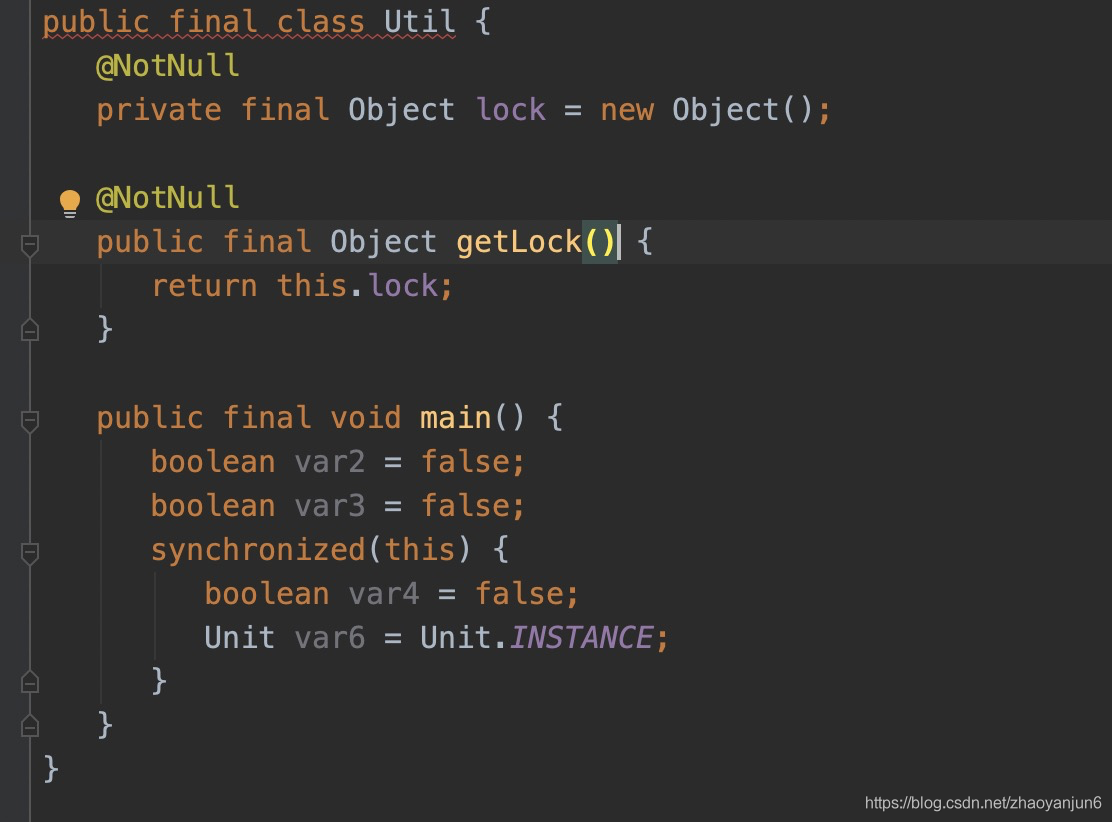
\includegraphics[width=.9\linewidth]{./pic/eg1.png}
\subsubsection{例子2}
\label{sec-5-2-2}
\begin{minted}[frame=lines,fontsize=\scriptsize,linenos=false]{kotlin}
class Util {
    val lock = Any()
    fun main() {
        synchronized(lock) {
        }
    }
}
\end{minted}
\begin{itemize}
\item 编译成 java 如下
\end{itemize}

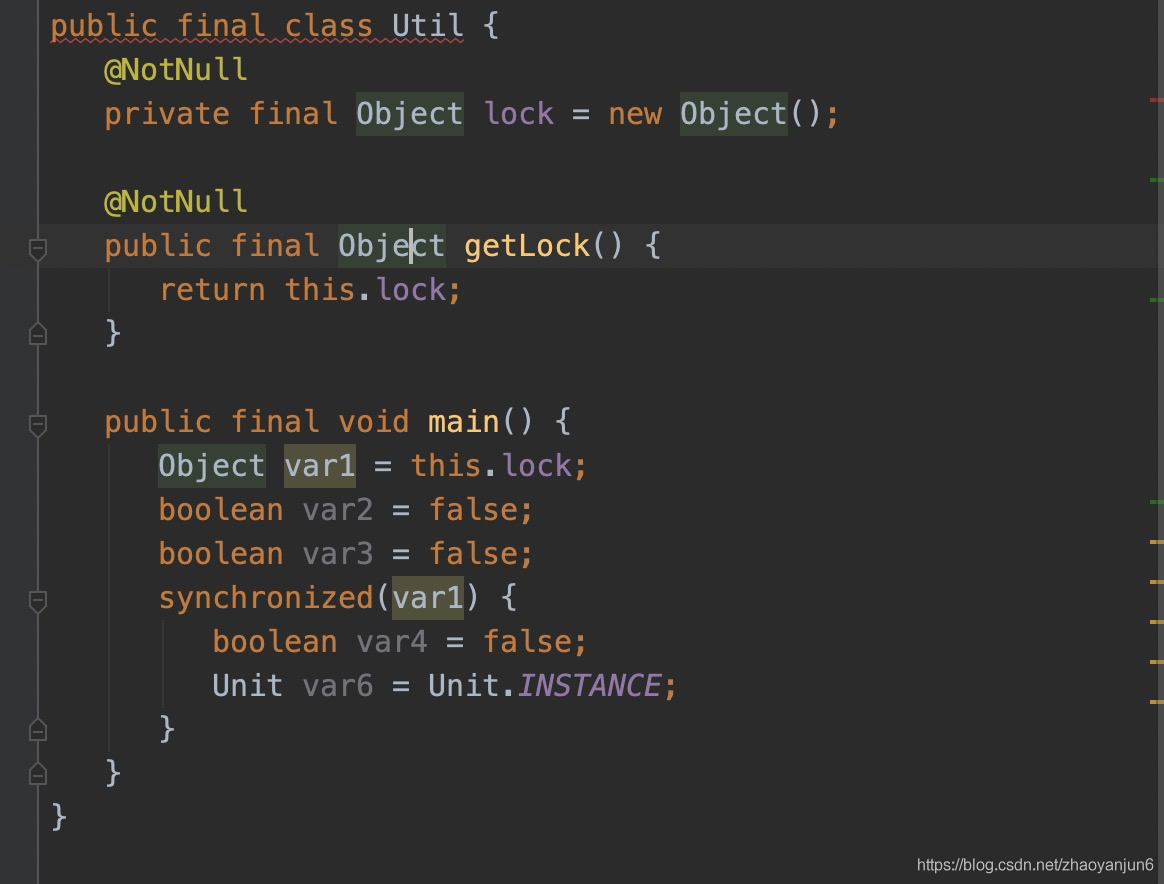
\includegraphics[width=.9\linewidth]{./pic/eg2.png}

\subsection{Volatile 关键字}
\label{sec-5-3}
\begin{itemize}
\item 在kotlin中没有volatile关键字,但是有 @Volatile 注解
\end{itemize}
\begin{minted}[frame=lines,fontsize=\scriptsize,linenos=false]{kotlin}
class Util {
    @Volatile
    var lock = Any()
}
\end{minted}
\begin{itemize}
\item 编译成 java 如下
\end{itemize}

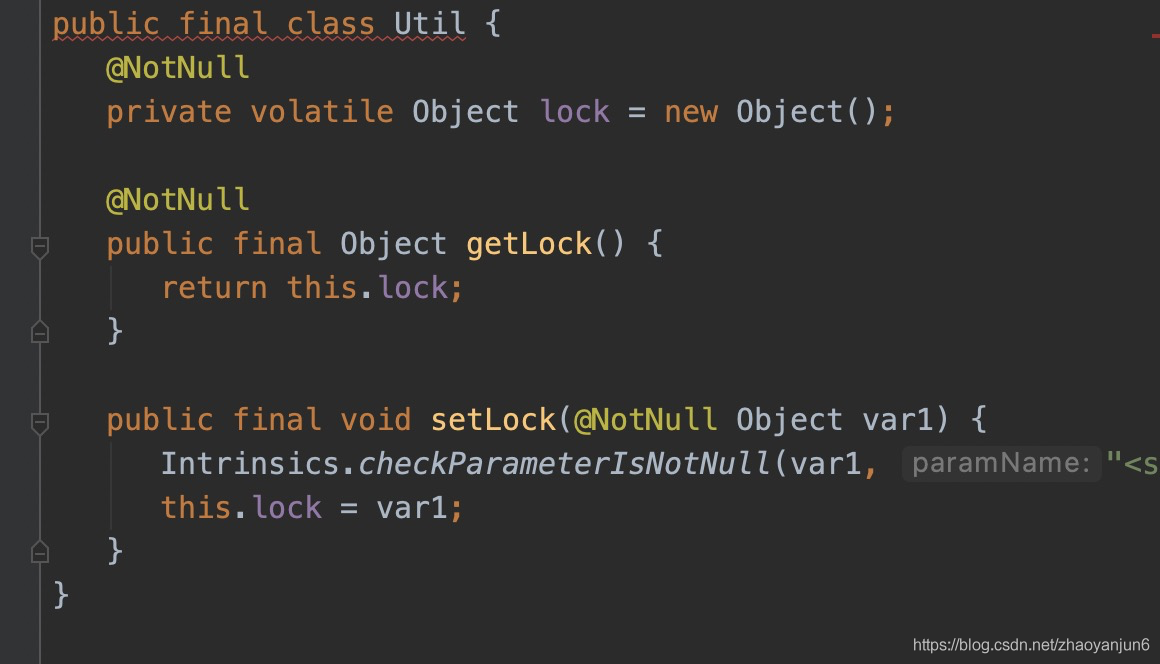
\includegraphics[width=.9\linewidth]{./pic/eg3.png}

\subsection{默认赋值}
\label{sec-5-4}
\subsubsection{默认不为空}
\label{sec-5-4-1}
\begin{minted}[frame=lines,fontsize=\scriptsize,linenos=false]{kotlin}
class A(val name: String, val age: Int)
\end{minted}
\begin{itemize}
\item 代表 name、age 不能为 null , 转换成 java , 会看到在构造函数中会对 name 字段做 空校验。
\end{itemize}

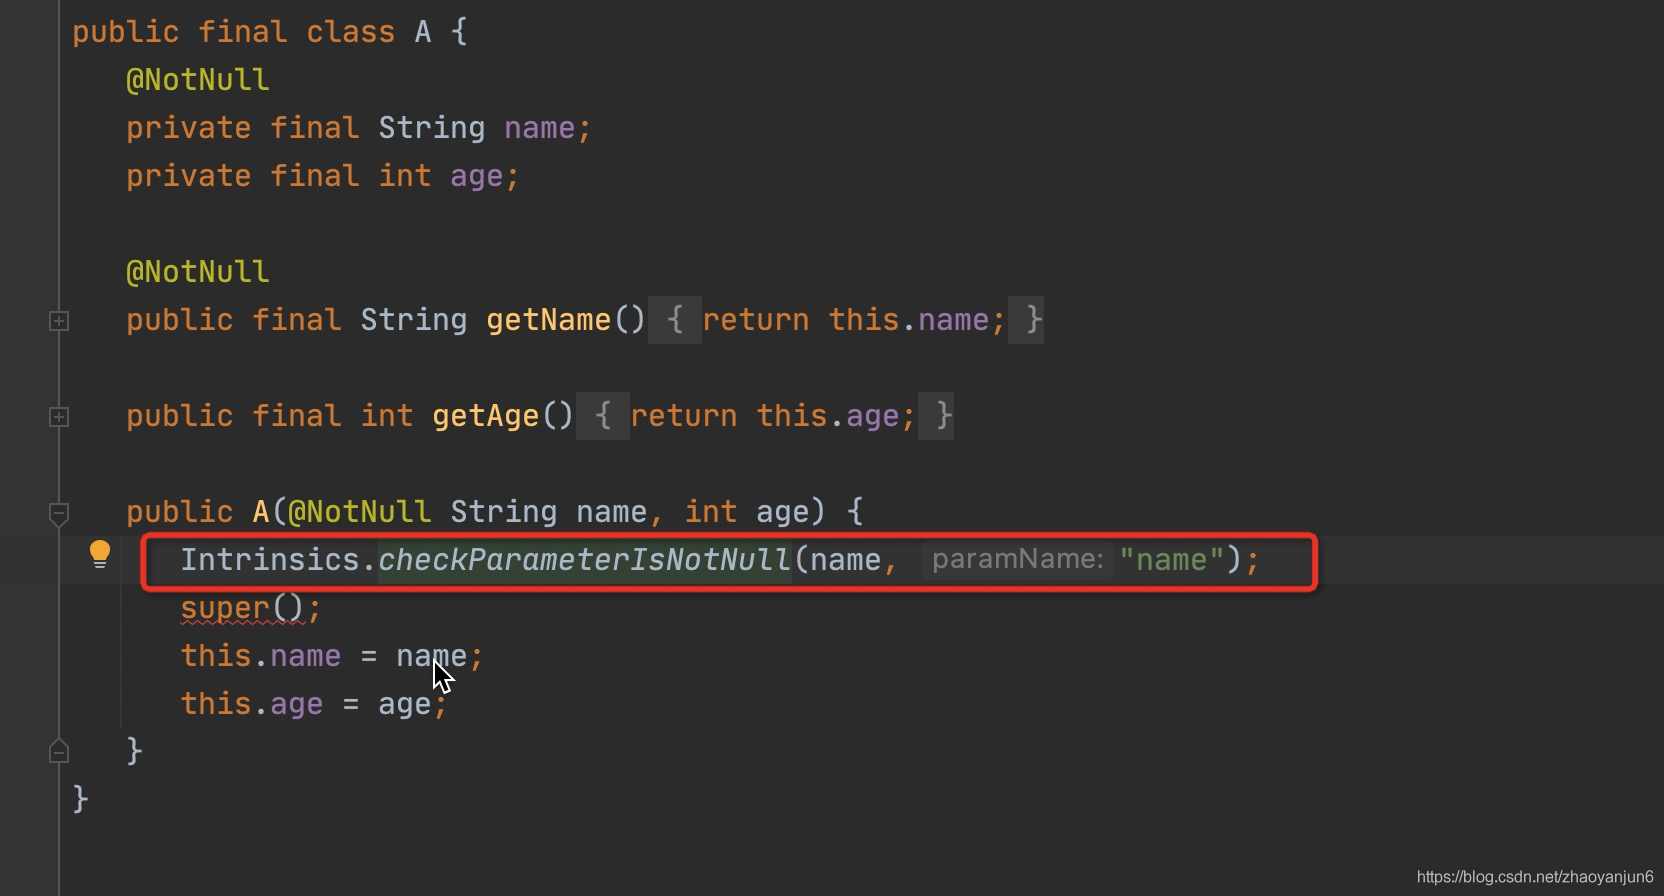
\includegraphics[width=.9\linewidth]{./pic/eg4.png}

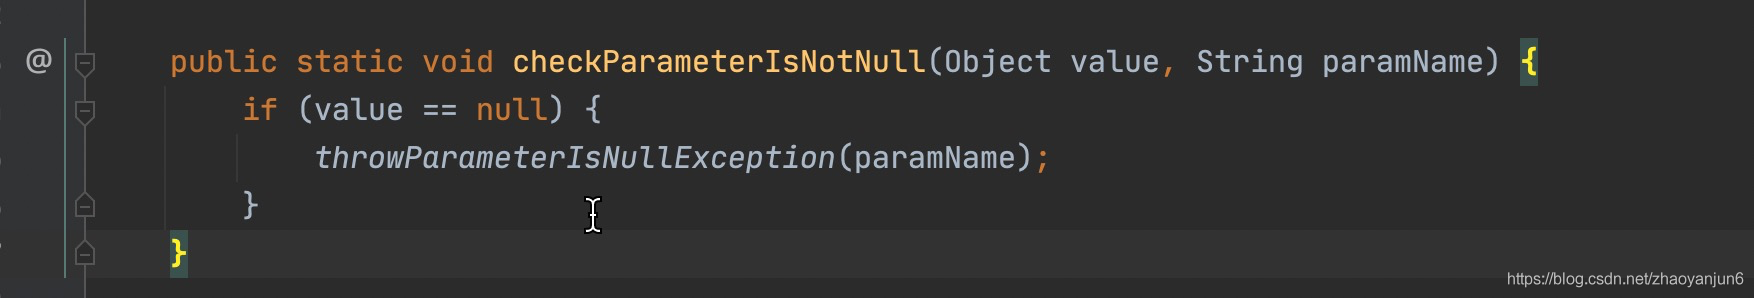
\includegraphics[width=.9\linewidth]{./pic/eg5.png}

\subsubsection{可以为空}
\label{sec-5-4-2}
\begin{minted}[frame=lines,fontsize=\scriptsize,linenos=false]{kotlin}
class A(val name: String?, val age: Int)
\end{minted}
\begin{itemize}
\item 代表 name 可为 null , 转换成 java , 会看到在构造函数中没有对 name 字段做 空校验。
\end{itemize}

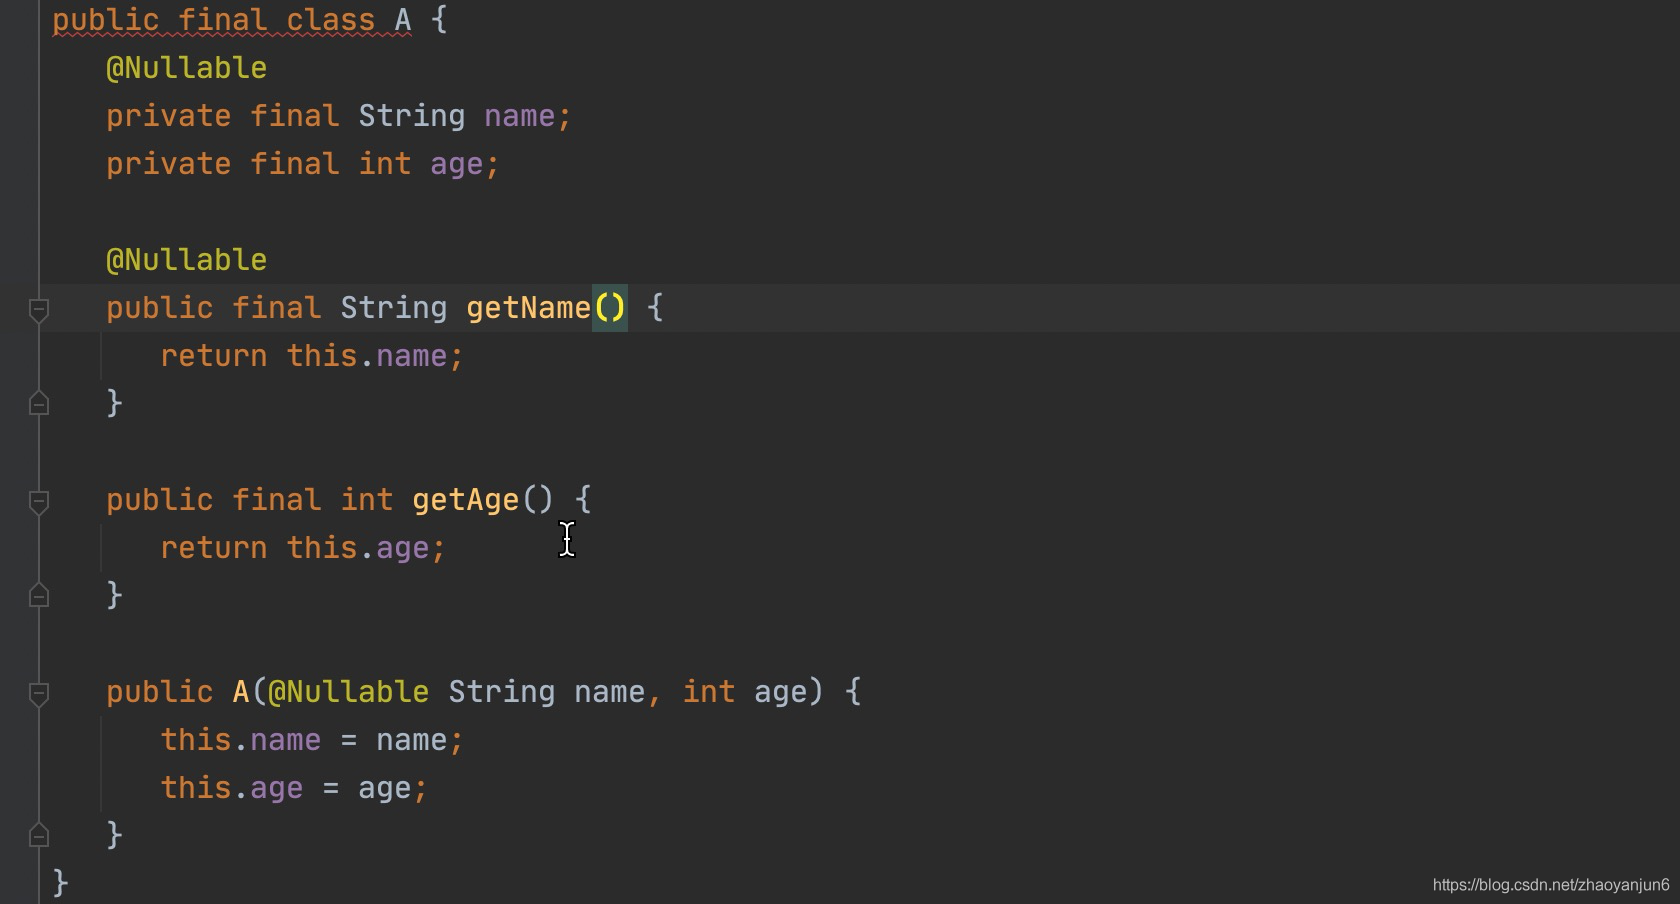
\includegraphics[width=.9\linewidth]{./pic/eg6.png}

\subsubsection{默认值}
\label{sec-5-4-3}
\begin{minted}[frame=lines,fontsize=\scriptsize,linenos=false]{kotlin}
class A(val name: String? = "zhaoyanjun", val age: Int)
\end{minted}
\begin{itemize}
\item name 可为空,如果name 为null, 使用默认值 “zhaoyanjun”
\end{itemize}

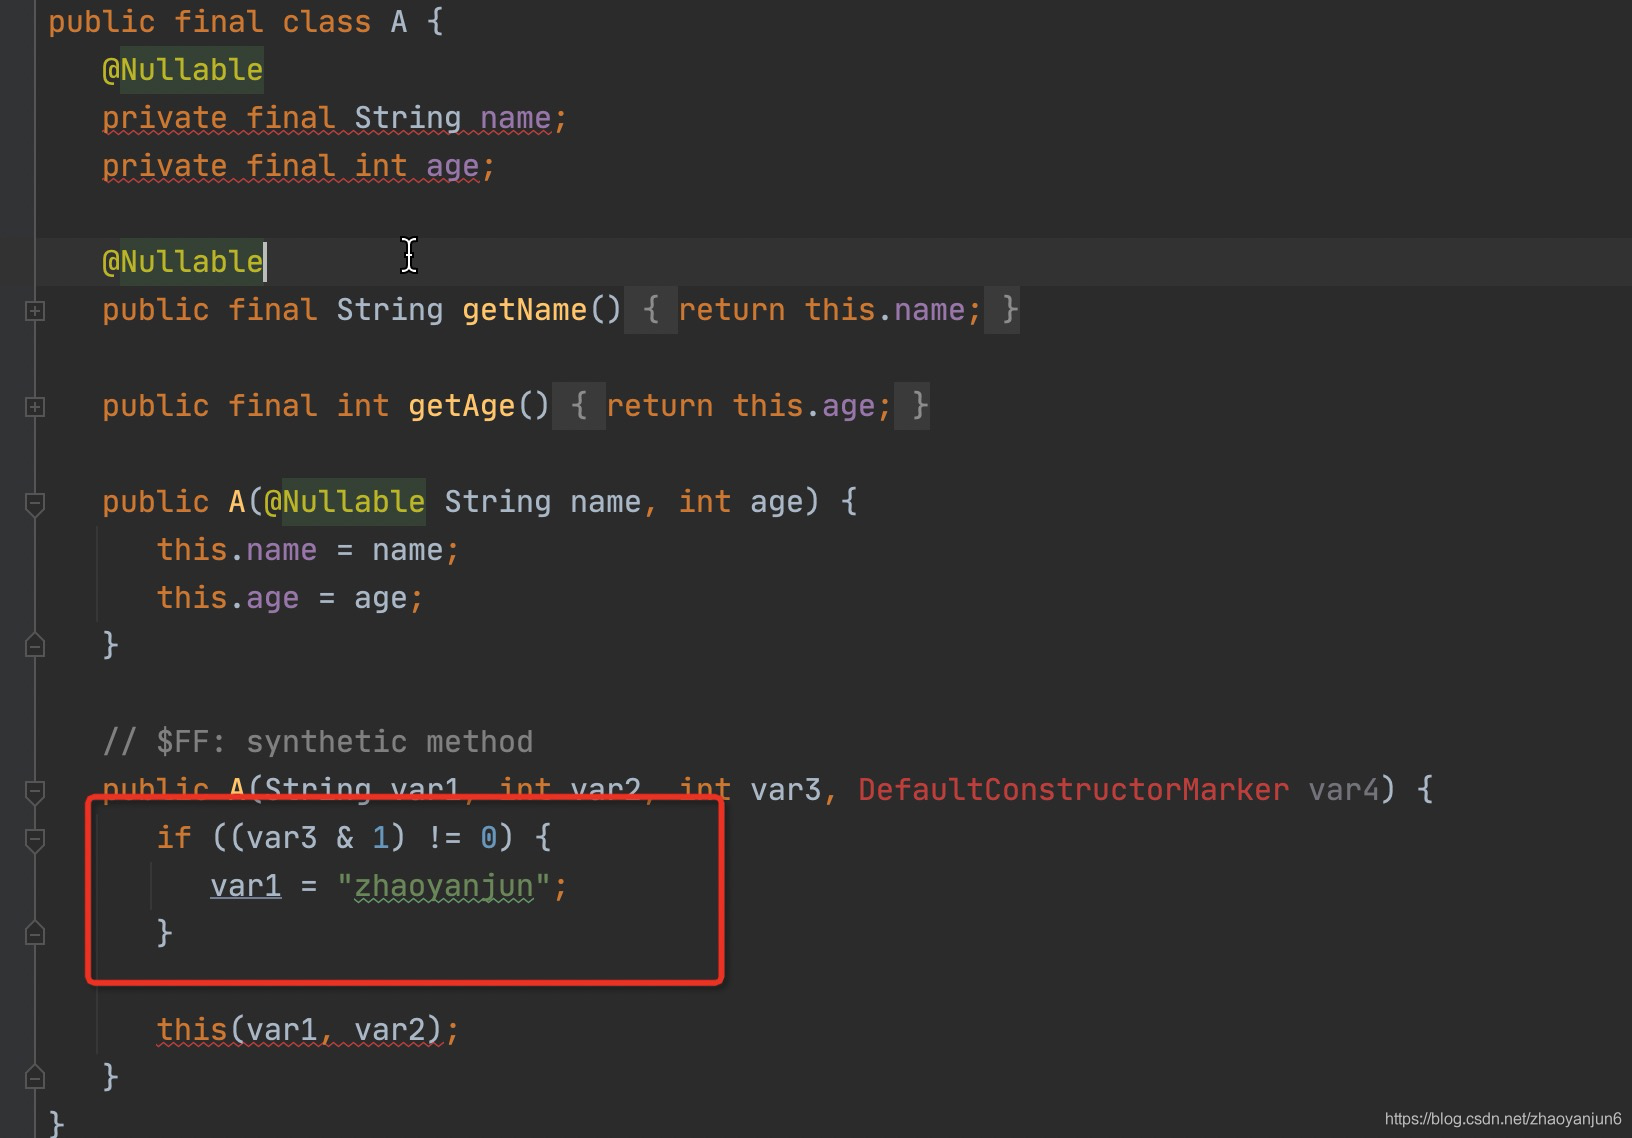
\includegraphics[width=.9\linewidth]{./pic/eg7.png}

\subsubsection{两个默认值}
\label{sec-5-4-4}
\begin{minted}[frame=lines,fontsize=\scriptsize,linenos=false]{kotlin}
class A(val name: String? = "zhaoyanjun", val age: Int ?= 10)
\end{minted}

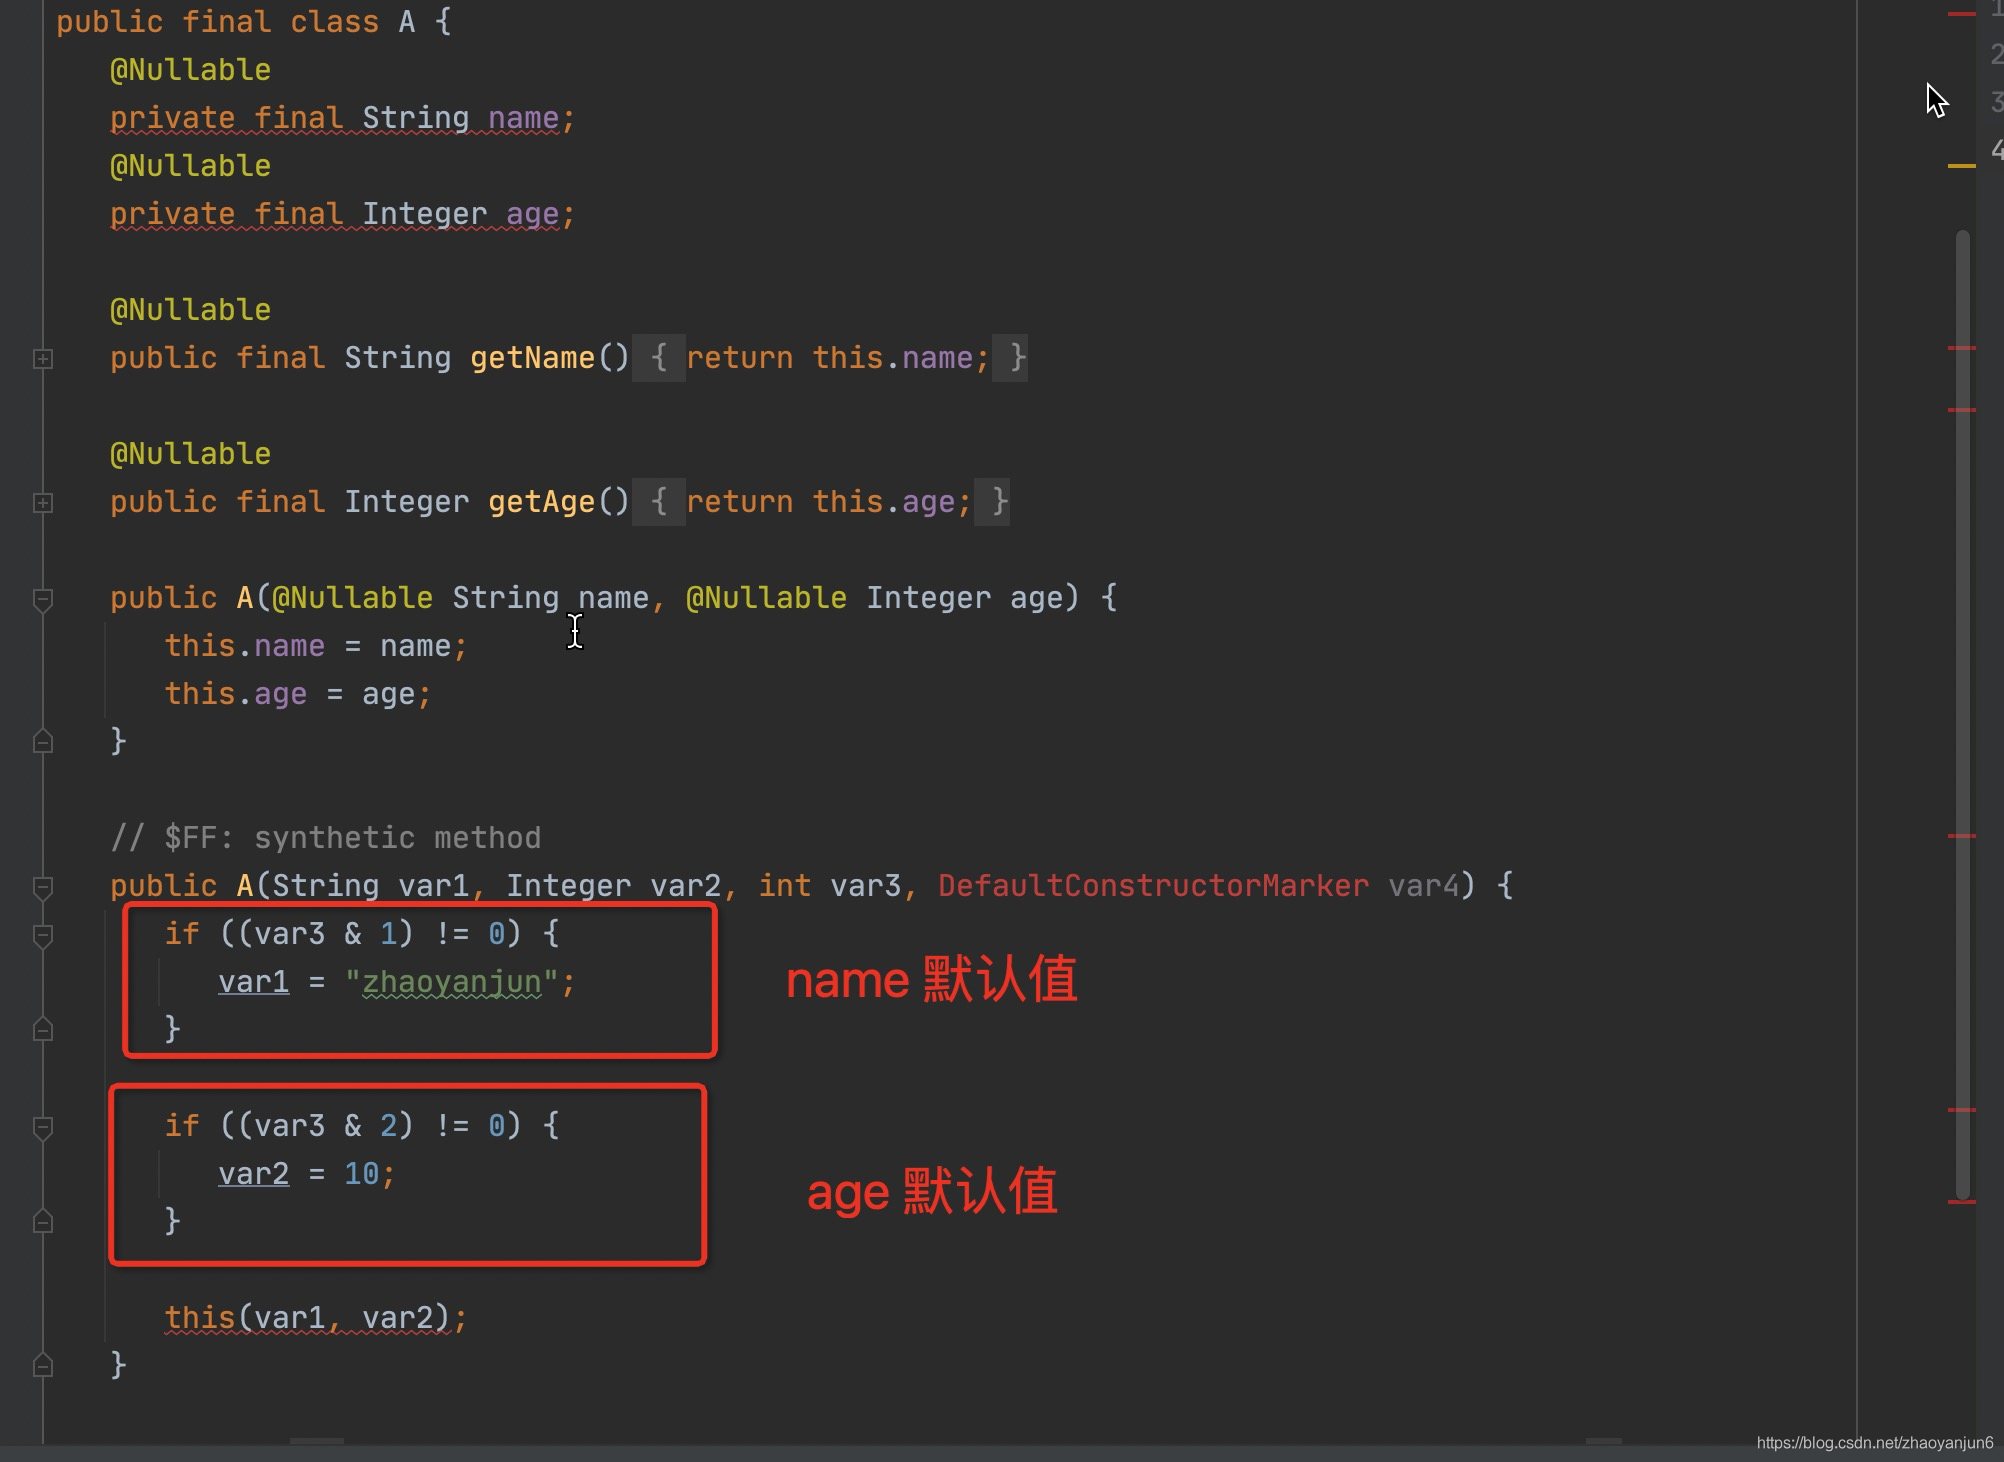
\includegraphics[width=.9\linewidth]{./pic/eg8.png}

\subsection{构造函数}
\label{sec-5-5}
\begin{minted}[frame=lines,fontsize=\scriptsize,linenos=false]{kotlin}
class A(val name: String, val age: Int)
var a1 =  A("zhaoyanjun",10)  //编译正常
var a =  A()  //编译失败,因为没有无参构造函数
\end{minted}

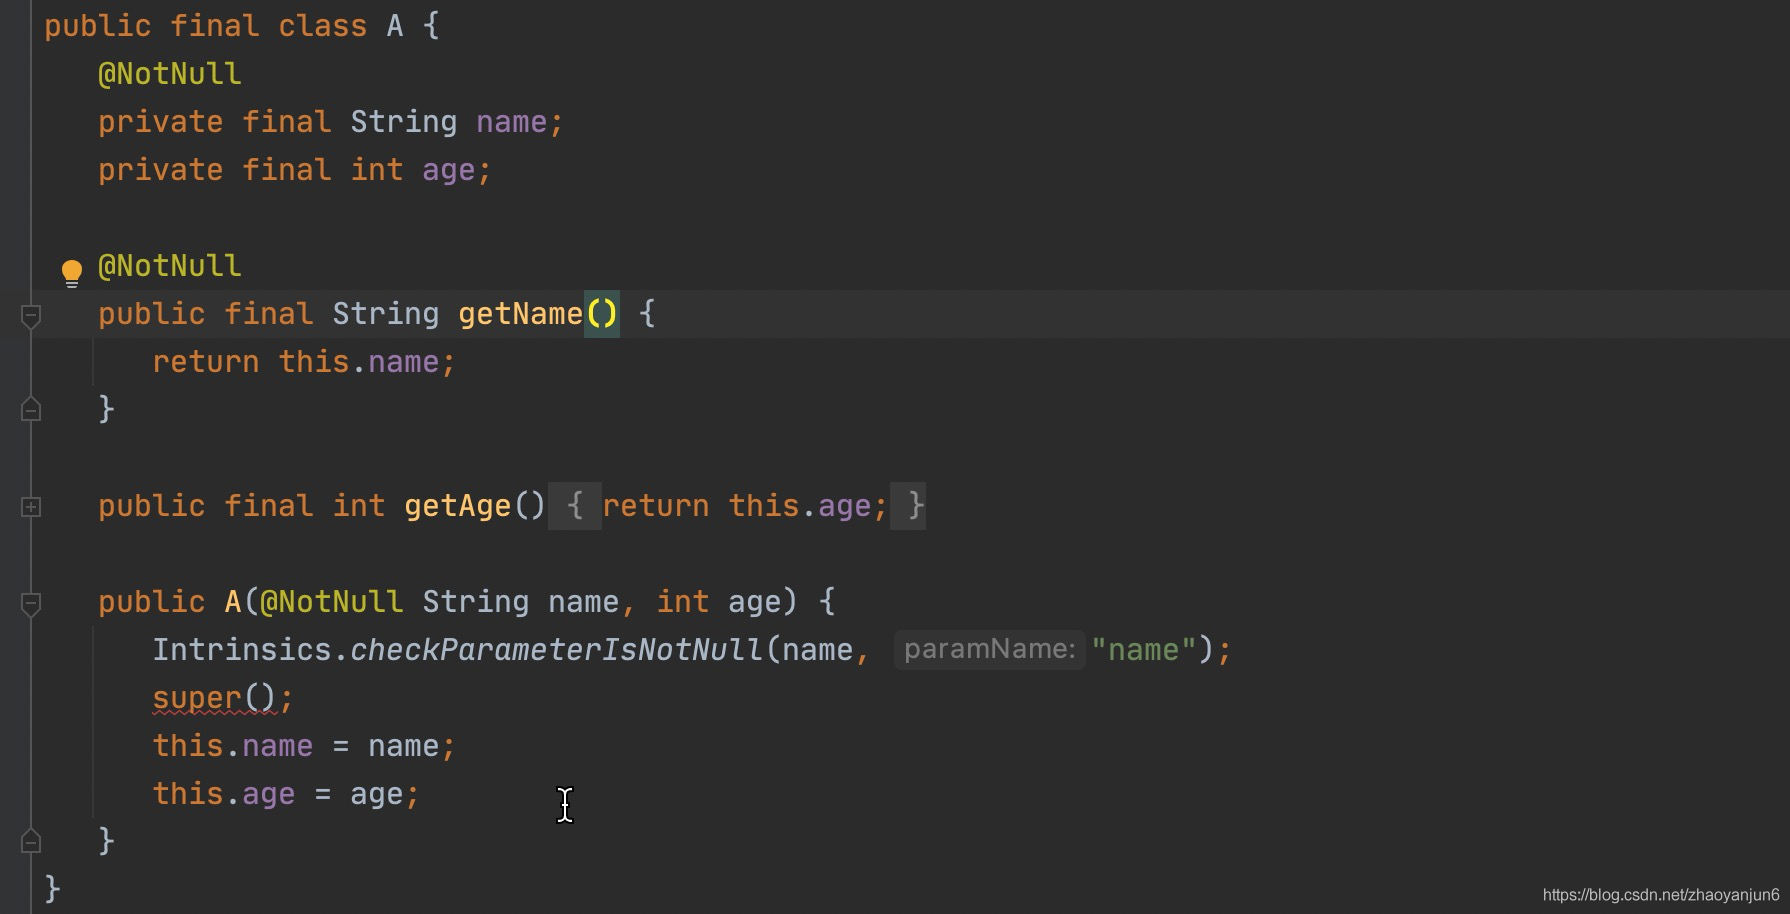
\includegraphics[width=.9\linewidth]{./pic/eg9.png}


\begin{itemize}
\item 如何才能调用无参构造函数呢?其实很简单,给每个参数添加一个默认值就可以了
\end{itemize}
\begin{minted}[frame=lines,fontsize=\scriptsize,linenos=false]{kotlin}
class A(val name: String? = "", val age: Int? = 0)
\end{minted}
\begin{itemize}
\item 只要参数都有默认值,就会默认生成 无参构造函数
\end{itemize}

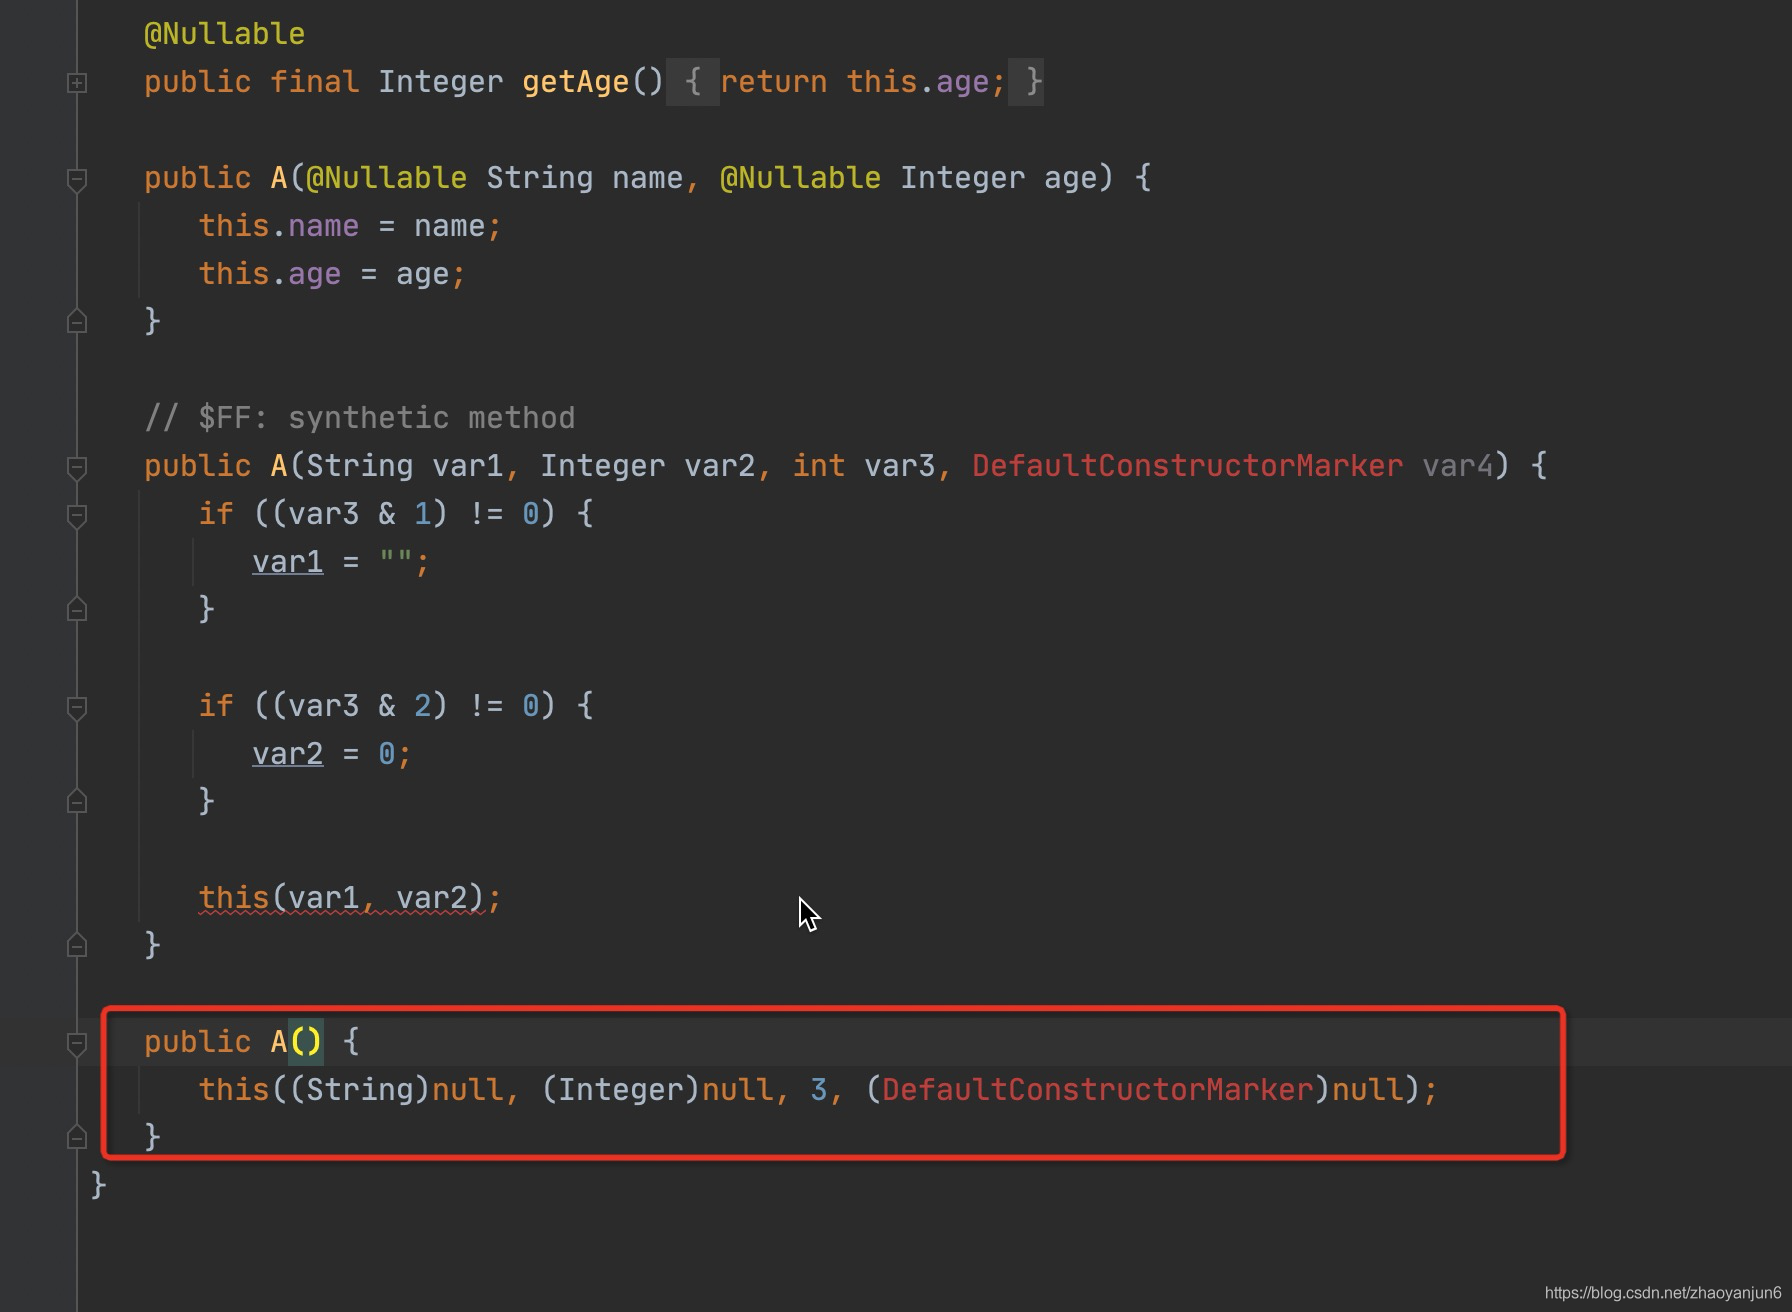
\includegraphics[width=.9\linewidth]{./pic/eg10.png}

\subsection{重载函数 @JvmOverloads}
\label{sec-5-6}
\begin{minted}[frame=lines,fontsize=\scriptsize,linenos=false]{kotlin}
class A(val name: String, val age: Int)
var a1 =  A("zhaoyanjun",10)   //编译正常
var a2 =  A("123")    //编译失败,没有只有一个参数的构造函数
\end{minted}
\begin{itemize}
\item 如何才能自动生成重载函数呢?其实很简单
\item 给每个参数添加默认值
\item 标记 constructor 关键字
\item 标记 @JvmOverloads 关键字
\end{itemize}
\begin{minted}[frame=lines,fontsize=\scriptsize,linenos=false]{kotlin}
class A @JvmOverloads constructor(val name: String? = "", val age: Int? = 0)
\end{minted}

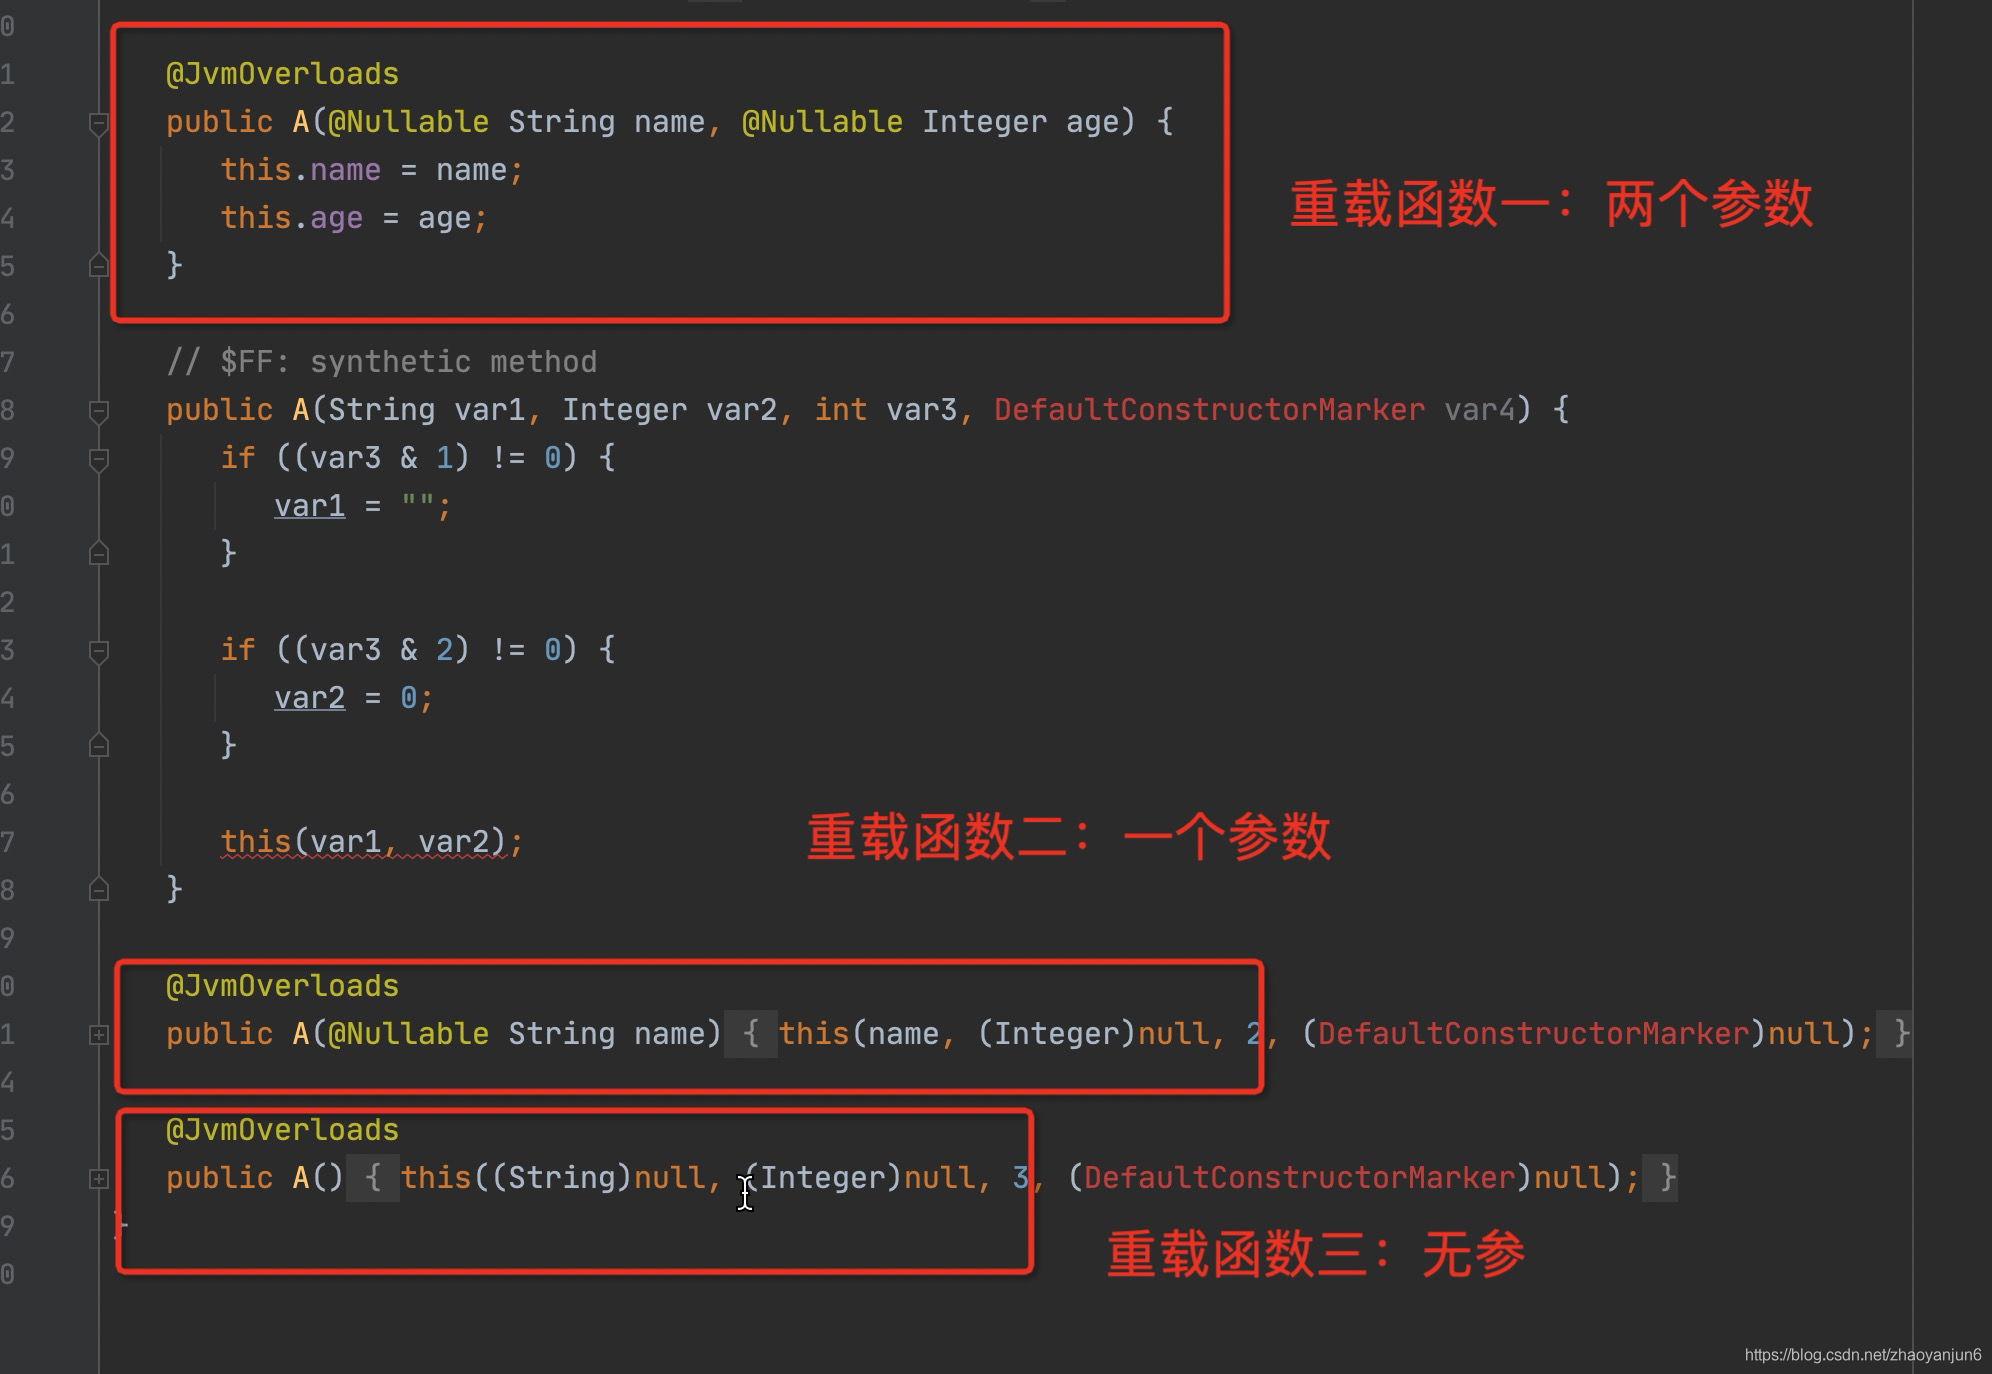
\includegraphics[width=.9\linewidth]{./pic/eg11.png}
% Emacs 27.1 (Org mode 8.2.7c)
\end{document}